\begin{figure}
\pgfplotsset{every x tick label/.append style={font=\tiny, rotate=30}}
\pgfplotsset{every y tick label/.append style={font=\tiny}}
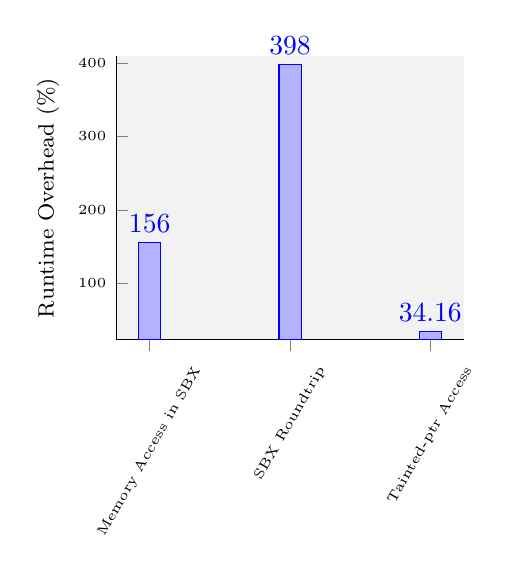
\begin{tikzpicture}  
  
\begin{axis}  
[  
    ybar,  
    %ymode=log,
    enlargelimits=0.03,
    enlarge x limits=0.12,
    ylabel={Runtime Overhead (\%)}, % the ylabel must precede a # symbol.  
     axis x line*=bottom,
     axis y line*=left,
    %xlabel={Micro-Benchmark Tests},  
    symbolic x coords={Memory Access in SBX, SBX Roundtrip, Tainted-ptr Access}, % these are the specification of coordinates on the x-axis.  
    xtick=data,  
    bar width=8pt,
    width=6cm,
    x tick label/.append style={font=\tiny, rotate=30},
    y tick label/.append style={font=\tiny},
    axis background/.style={fill=gray!10},
    x label style={at={(axis description cs:0.5,-0.1)},anchor=north, font=\footnotesize},
    xlabel={},
    ylabel style={font=\footnotesize},
     nodes near coords, % this command is used to mention the y-axis points on the top of the particular bar.  
    nodes near coords align={vertical},  
    ]  
\addplot coordinates {(Memory Access in SBX,156) (SBX Roundtrip, 398) (Tainted-ptr Access, 34.16)};  
  
\end{axis}  
\end{tikzpicture} 
\vspace*{-1.5em}
\caption{\systemname Micro-Benchmarks.}
\label{fig:microbenchmarks}

\pgfplotsset{every x tick label/.append style={font=\tiny, rotate=30}}
\pgfplotsset{every y tick label/.append style={font=\tiny}}
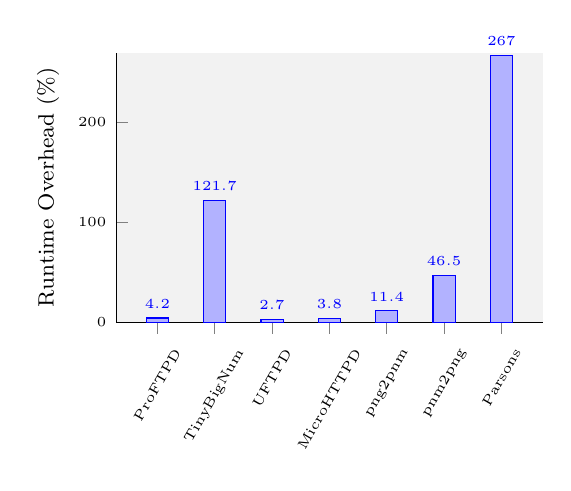
\begin{tikzpicture}  
  
\begin{axis}  
[  
    ybar = 0.8,  
    enlargelimits=0.01,  
    enlarge x limits=0.12,
    ylabel={Runtime Overhead (\%)}, % the ylabel must precede a # symbol.  
     axis x line*=bottom,
     axis y line*=left,
    %xlabel={Programs},  
    symbolic x coords={ProFTPD, TinyBigNum, UFTPD, MicroHTTPD, png2pnm, pnm2png, Parsons}, % these are the specification of coordinates on the x-axis.  
    xtick=data,  
    bar width=8pt,
    %legend style={font=\tiny},
    legend style={font=\tiny, at={(0.7,1.0)}},
    width=7cm,
    height=5cm,
    x tick label/.append style={font=\tiny, rotate=30},
    y tick label/.append style={font=\tiny},
    axis background/.style={fill=gray!10},
    x label style={at={(axis description cs:0.5,-0.1)},anchor=north, font=\tiny},
    xlabel={},
    ylabel style={font=\footnotesize},
    every node near coord/.append style={font=\tiny},
     nodes near coords, % this command is used to mention the y-axis points on the top of the particular bar.  
    nodes near coords align={vertical},  
    ]  
\addplot coordinates {(ProFTPD,4.2) (TinyBigNum,121.7) (UFTPD, 2.7) (MicroHTTPD,3.8) (png2pnm, 11.4) (pnm2png, 46.5) (Parsons, 267)};  

  
\end{axis}  
\end{tikzpicture} 
\vspace*{-1.5em}
\caption{Runtime Overhead of Partioned Programs.}
\label{fig:runtimeoverhead}
\end{figure}

